\textbf{Creación de Máquina Virtual}
\begin{enumerate}

\item En primer lugar, elegimos el nombre de la máquina: \textbf{Atacante01} y el tipo, en este caso se trata de \textbf{Linux} versión Kali Linux 2019.3, como esta opción no está disponible elegimos \textbf{Other Linux (64-bit)}.
\begin{figure}[H] %[H] para here [b] para bottom [t] para top
\begin{center}
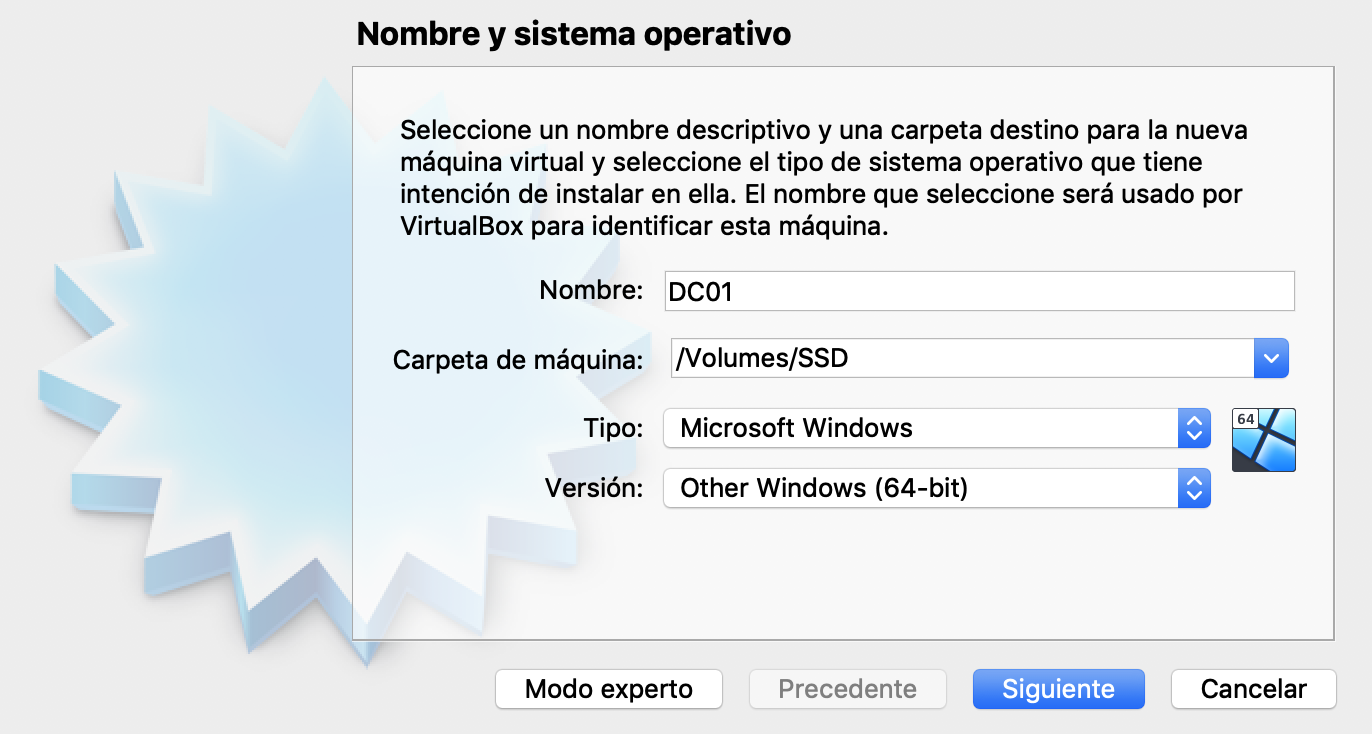
\includegraphics[width=10cm]{Atacante01/MV1.png}
\end{center}
\end{figure}

\item En el segundo paso, elegimos la RAM que vamos a destinar a la máquina virtual, al tratarse de la máquina donde se van a realizar las pruebas se destinan 4GB: \textbf{4096 MB}.
\begin{figure}[H] %[H] para here [b] para bottom [t] para top
\begin{center}
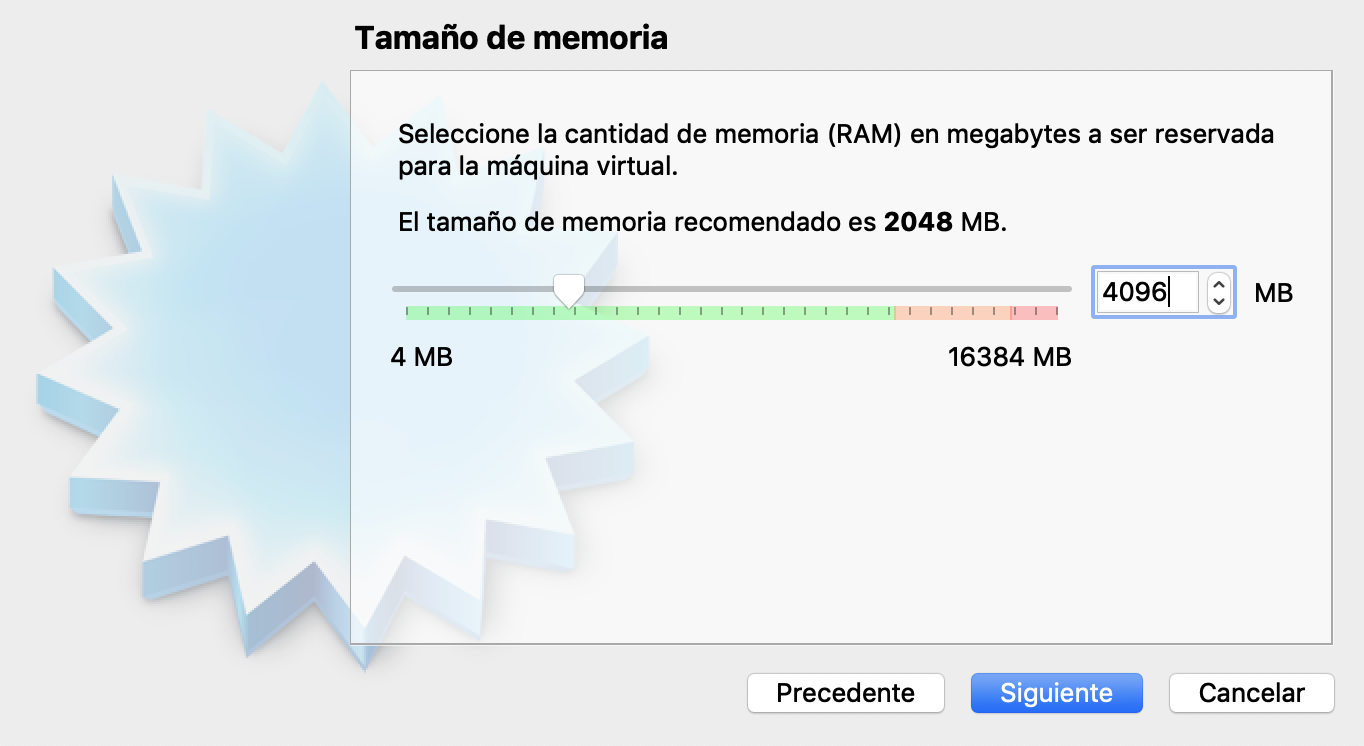
\includegraphics[width=10cm]{Atacante01/MV2.png}
\end{center}
\end{figure}

\item En esta opción, se elige \textbf{Crear un disco duro virtual ahora}.
\begin{figure}[H] %[H] para here [b] para bottom [t] para top
\begin{center}
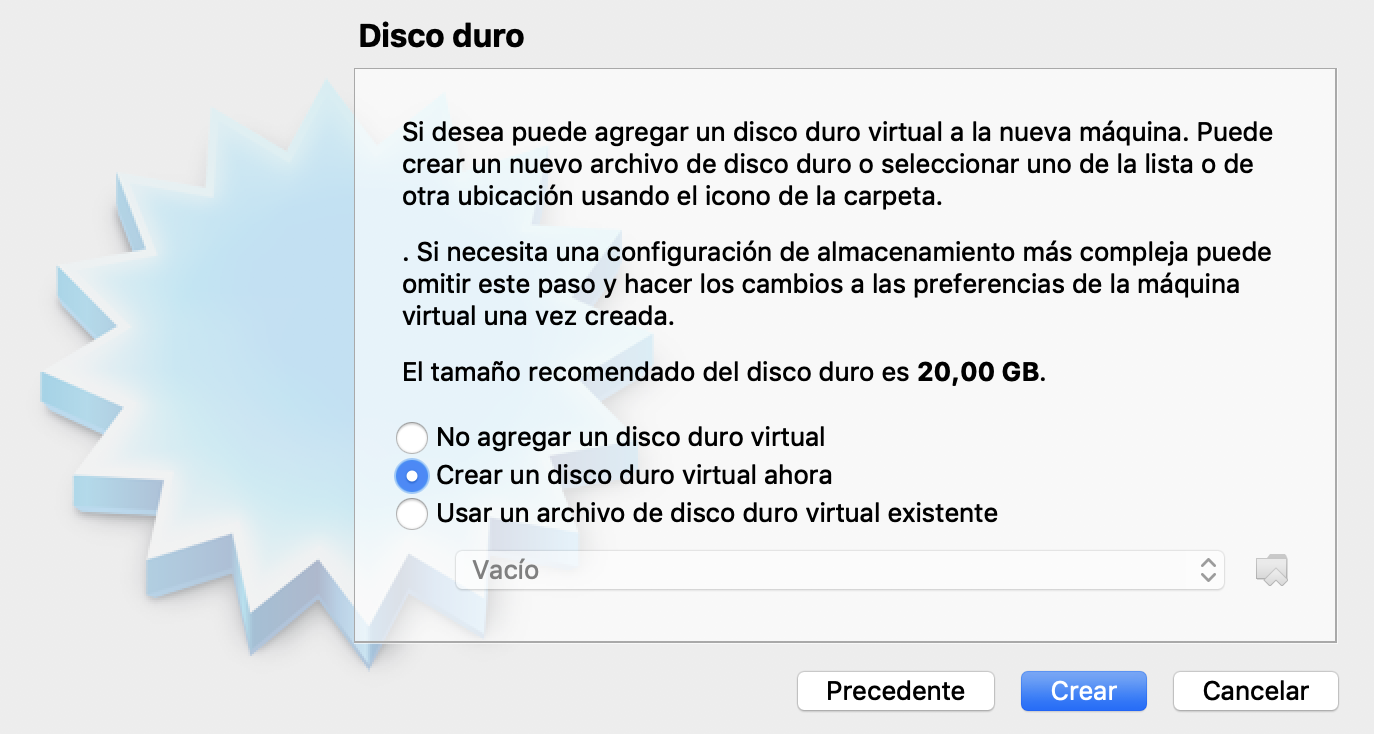
\includegraphics[width=10cm]{Atacante01/MV3.png}
\end{center}
\end{figure}

\item En cuanto al tipo de disco duro virtual se elige \textbf{VDI (Virtualbox Disk Image)}.
\begin{figure}[H] %[H] para here [b] para bottom [t] para top
\begin{center}
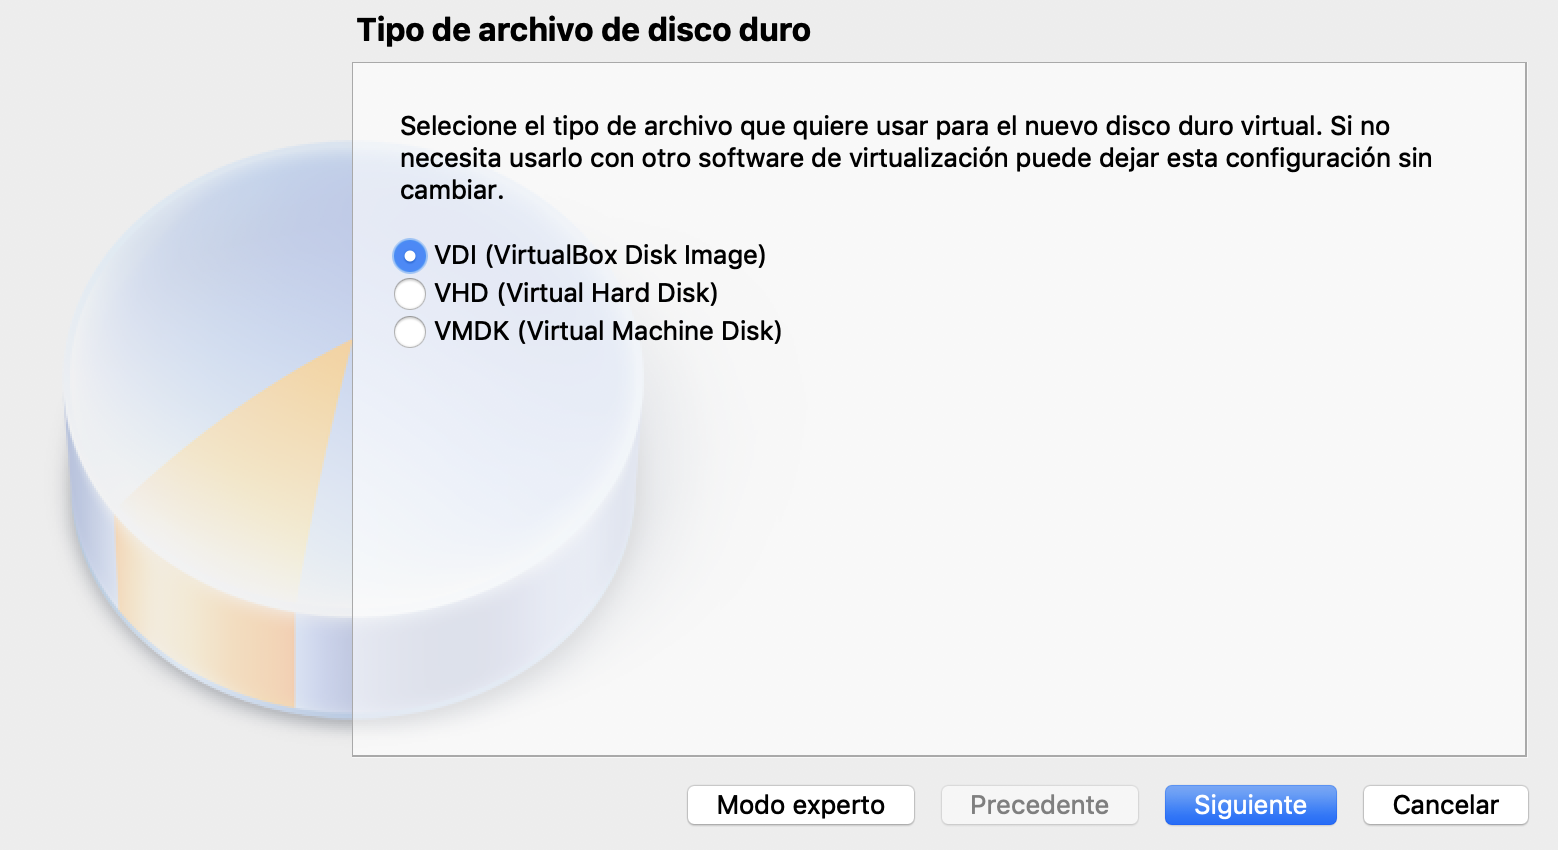
\includegraphics[width=10cm]{Atacante01/MV4.png}
\end{center}
\end{figure}

\item Por último, se ha elegido \textbf{15 GBs} de espacio de disco duro virtual.
\begin{figure}[H] %[H] para here [b] para bottom [t] para top
\begin{center}
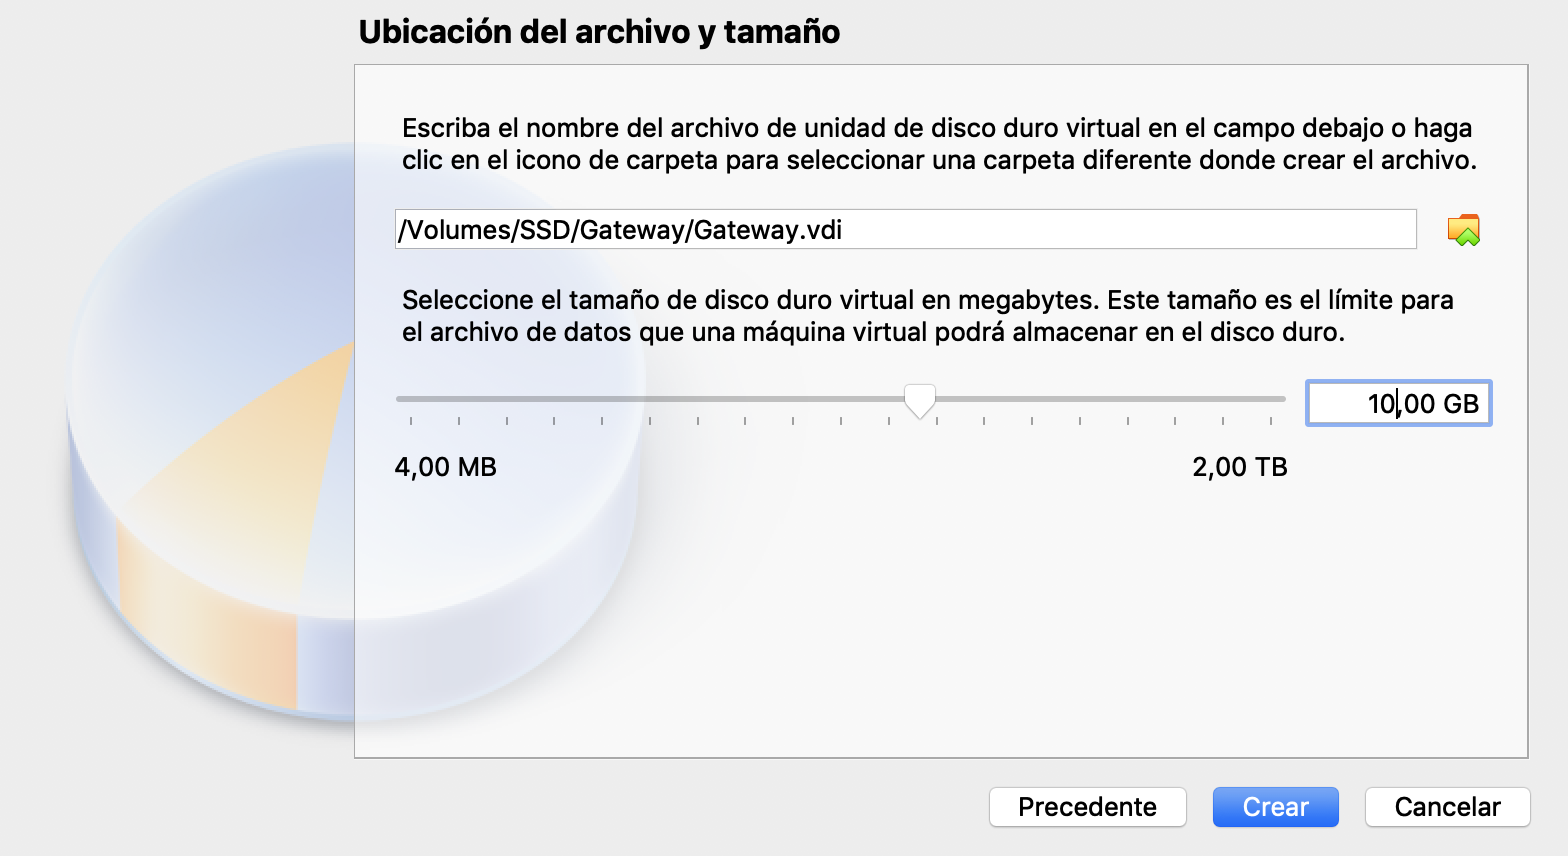
\includegraphics[width=10cm]{Atacante01/MV5.png}
\end{center}
\end{figure}

\item Para arrancar la imagen del sistema operativo, hay que seleccionarla desde Con\-fi\-gu\-ra\-ción/\-Almacenamiento de la máquina virtual creada como Unidad Óptica.
\begin{figure}[H] %[H] para here [b] para bottom [t] para top
\begin{center}
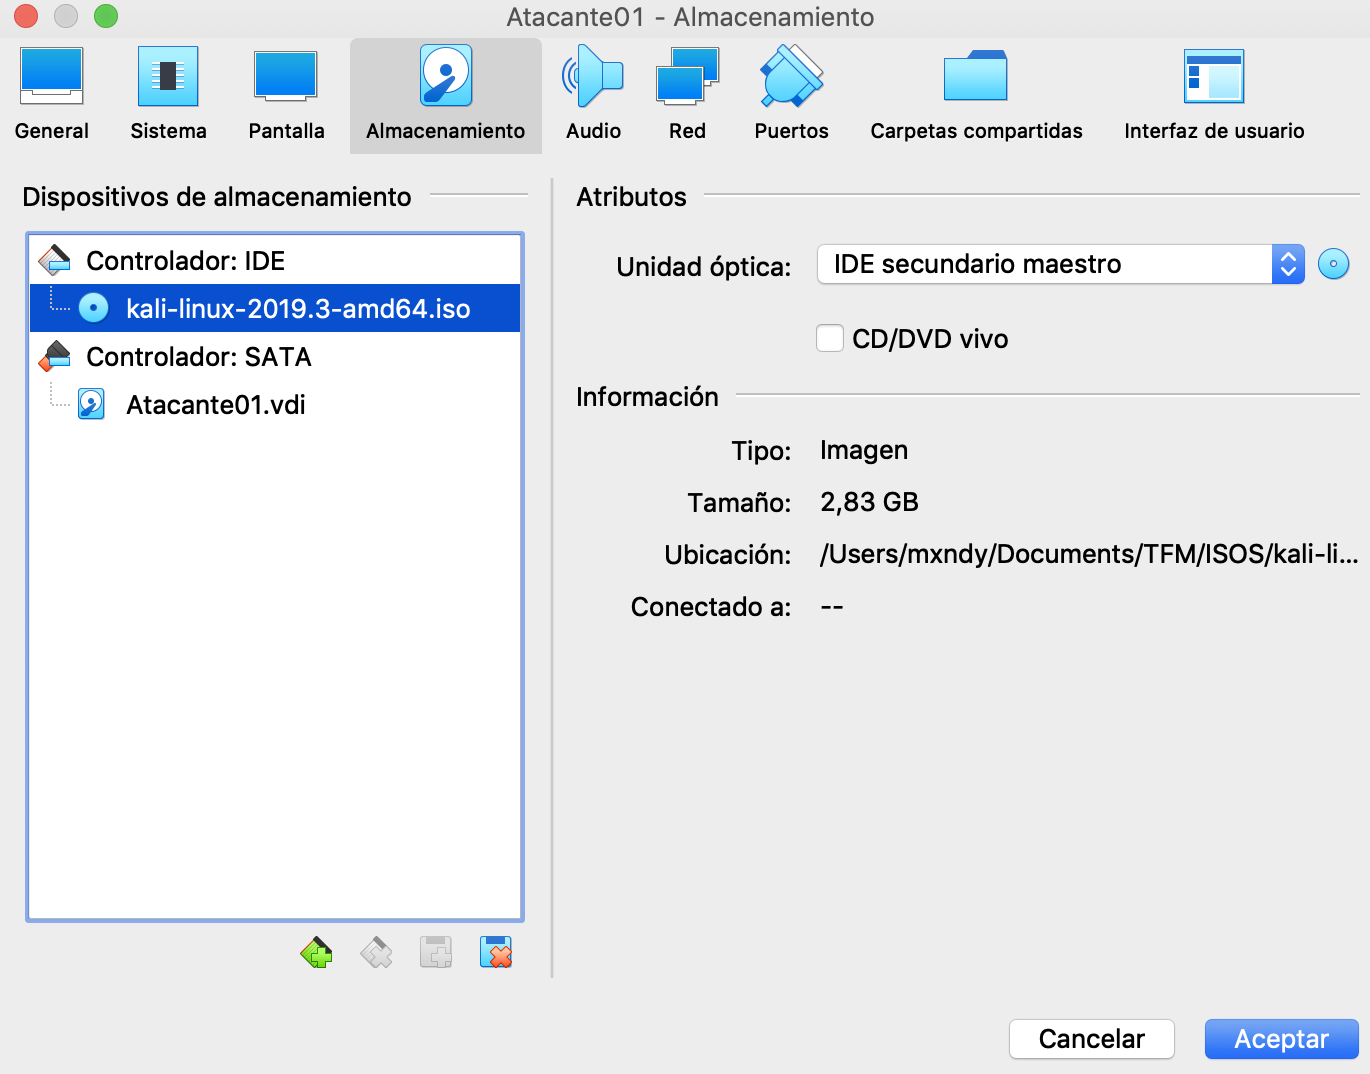
\includegraphics[width=10cm]{Atacante01/MV6.png}
\end{center}
\end{figure}




\end{enumerate}
\textbf{Instalación}

\textbf{Actualización}
